\chapter{Projectmanagement}

\section{Introduction}

\subsubsection*{Purpose of this document}
This chapter shows the project plan for the bachelor thesis "Functional Kafka".
It is used as basis for the planning during the work. 

\subsubsection*{Goal of the project}
Analyzing Apache Kafka, a state of the art message broker system created at
LinkedIn and adapt basic features to build an alternative broker system in
Haskell. 

\section{Organization}

\subsubsection*{Structure}

\begin{tabular}[t]{|l|l|l|} \hline
\textbf{Name} & \textbf{E-mail} & \textbf{Responsibility} \\ \hline
Marc Juchli & mjuchli@hsr.ch & Research, Development, Documentation \\ \hline
Lorenz Wolf & l1wolf@hsr.ch & Research, Development, Documentation \\ \hline 
\end{tabular}

\subsubsection*{Externe Schnittstellen}

\begin{tabular}[t]{|l|l|l|} \hline
\textbf{Name} & \textbf{E-Mail} & \textbf{Responsibility}  \\ \hline
Prof Dr. Josef Joller & jjoller@hsr.ch & Supervisor \\ \hline 
Dr. Simon Meier & simon.y.meier@gmail.com & Expert  \\ \hline\end{tabular}

%\subsubsection*{Sitzungen}

%\begin{itemize}
%\item 
%\end{itemize}
\newpage
\section{Planning}
We separated the work in three phases inception, elaboration and construction
(adapted from Rational Unified Process, RUP). For planning the time schedule we
first defined tasks very rough granular. For each of those we then planed
subtasks which can be seen as single issues (see \ref{subsec:tasks}).
Furthermore three milestones were set to define particular objectives we want to
achieve at a specific time (see table \ref{tab:MeilensteineZiele}).  After reaching the
planed end of a milestone, a set-actual comparison is made (see
\ref{sec:status-tracking}). Performed work is
tracked via an Atlassian JIRA platform where we manage tasks for the project.
Specific issues are tracked and managed via GitHub Repository. 


\subsection{Time schedule}
\begin{figure}[H]
    \centering
    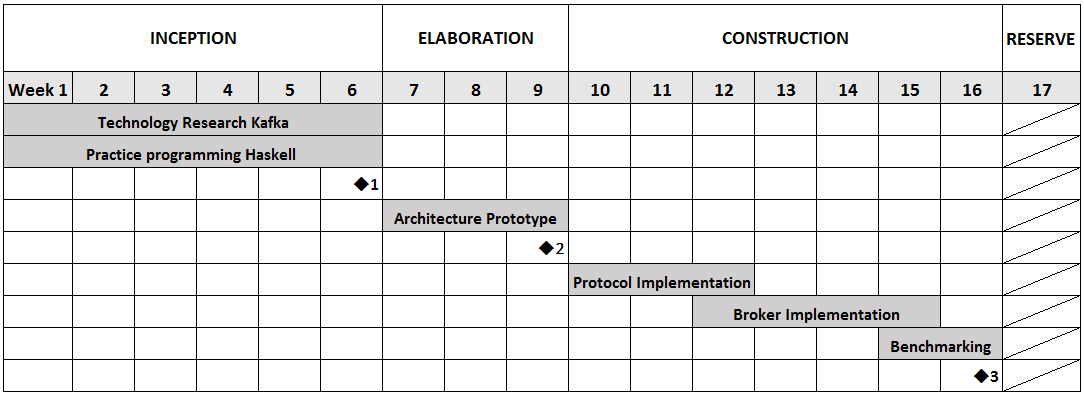
\includegraphics[width=1\textwidth]{images/workschedule.png}
    \caption{Time schedule, GANTT style}
    \label{fig:workschedule}
\end{figure}

\subsection{Milestones}
\begin{tabular}[H]{|p{4cm}|l|p{4.5cm}|p{4.5cm}|}\hline
    \textbf{Milestone} & \textbf{Deadline} & \textbf{Objectives} & \textbf{Deliverables} \\ \hline
    M0 Start of work & 16.02.2015 & - & -\\ \hline
    M1 Completion of research  & 22.03.2015 & 
        Necessary background knowledge about Kafka related topics as well as
        Haskell skills are ready for implementation part. 
        &
        Documentation technology research \\ \hline
    M2 End of elaboration & 19.04.2015 & 
        After a period of three weeks we want to have a concept and first running
        code to show some basic functionality and feasibility. 
        &
        Architecture prototype \\ \hline
    M3 End of construction & 07.06.2015 & 
        Code freeze, all planned features are implemented. Broker runs stable and
        benchmark results exist. 
        &
        Stable broker and protocol implementation. Benchmarks results. Technical
        report.\\ \hline
  %\begin{itemize}
  %  \item \ldot
  %\end{itemize} \\ \hline
\end{tabular}
\captionof{table}{Milestones and their objectives}
\label{tab:MeilensteineZiele}

\newpage
\subsection{Tasks}
\label{subsec:tasks}
\subsubsection{Inception}


\begin{tabular}[H]{|p{6cm}|p{10cm}|}\hline
    \textbf{Task} & \textbf{Subtasks} \\ \hline
    Technology Research Kafka & 
        \begin{itemize}
            \item Learn Messaging and Event Streaming fundamentals.
            \item Analyse Apache Kafka and related topics. 
            \item Write research documentation.
        \end{itemize} \\ \hline
    Practice programming Haskell & 
        \begin{itemize}
            \item Familiarize with the functional paradigm.
            \item Setup developer environment. 
            \item Learn Haskell as functional programming language.
            \item Become acquainted to libraries regarding networking,
              building server application, and serialization.
        \end{itemize} \\ \hline
\end{tabular}
\captionof{table}{Tasks of inception phase}

\subsubsection{Elaboration}
\begin{tabular}[H]{|p{6cm}|p{10cm}|}\hline
   \textbf{Task} & \textbf{Subtasks} \\ \hline
    Architecture Prototype &
        \begin{itemize}
            \item Set up basic server architecture.
            \item Set up concept for implementing the wire protocol.
            \item Implement basic message workflow from producing messages to
            persisting at broker.
            \item Implement simplified clients to demonstrate architecture
                prototype prototype.
        \end{itemize} \\ \hline
   \end{tabular}
\captionof{table}{Tasks of elaboration phase}

\subsubsection{Construction}
\begin{tabular}[H]{|p{6cm}|p{10cm}|}\hline
   \textbf{Task} & \textbf{Subtasks} \\ \hline
    Protocol Implementation &
        \begin{itemize}
            \item Work out details of protocol implementation. Finish
                implementation of relevant parts for producing and consuming
                messages. 
            \item Implement client API for exposing simplified access to protocol
                implementation.
            \item Ensure and test Kafka compatibility.
        \end{itemize} \\ \hline
    Broker Implementation &
        \begin{itemize}
            \item Work out details of server application.
            \item Develop message log persistency adapt from Apache Kafka. 
            \item Optimizations to approximate performance approach of
            Apache Kafka. 
        \end{itemize} \\ \hline
    Benchmarking &
        \begin{itemize}
            \item Define reasonable benchmarks.
            \item Test resulting broker implementation for performance.
            \item Comparing performance with Apache Kafka.
        \end{itemize} \\ \hline
\end{tabular}
\captionof{table}{Tasks of construction phase}

Last week of the schedule is reserved for completion work and documentation. 

\newpage
\section{Risk management}

In the table \ref{tab:Risiken} are the risk which could influence our thesis: 

\begin{tabular}[t]{|p{3cm}|p{3cm}|r|r|r|p{3cm}|p{3cm}|}\hline
\textbf{Risk} &
    \textbf{Impact} &
  \begin{sideways} \textbf{Probability } \end{sideways} &
  \begin{sideways}\textbf{Loss} \end{sideways} &
  \begin{sideways}\textbf{Risk} \end{sideways} &
  \textbf{Prevention} & \textbf{Consequences} \\ \hline
    Missing know-how in new technology & 
    Slow progress, inefficiency & 
    0.9 & 
    0.1 & 
    0.3 & 
    Ask experts before spending to much time & 
    It is part of this thesis to learn new technologies, we expect decelerated
    progress from time to time but we can deal with it. \\ \hline
  Technical impossibility & 
    No resulting product, change to other technology, loss in time. & 
    0.1 & 
    0.9 & 
    0.1 & 
    Analyse possibilities before spending to much time . &
    Inform supervisor or expert.
    \\ \hline
\end{tabular}
\captionof{table}{Risks}
\label{tab:Risiken}

%Sollte trotz den vorbeugenden Massnahmen ein zeitlicher Schaden
%entstehen, muss die Projektplanung unter Umständen angepasst werden.
%Die Zeiterfassung wird von den Projektmitarbeitern in Redmine erfasst.
%Redmine ist über folgenden Link erreichbar:
%\url{http://152.96.56.42/redmine/}. Die Projektmitarbeiter haben einen
%persönlichen Zugang  um die Daten zu erfassen. Der Betreuer hat
%ebenfalls ein Zugang, mit welchem er die Fortschritte mitverfolgen kann.
%Auf Redmine ist der aktuelle Stand des Projekts zu sehen.


%\section{Qualitätsmanagement}

%Um die Arbeitsergebnisse qualitativ auf einem hohen Niveau zu halten,
%arbeiten die Projektmitglieder nach dem Vier-Augen-Prinzip. Ein Dokument
%wird immer von beiden durchgelesen. Allfällige Änderungen werden gleich
%bilateral diskutiert und allenfalls angebracht. Somit soll erreicht
%werden, dass beide Projektmitglieder mit den Ergebnissen einverstanden
%und zufrieden sind.  Um Programmieraufgaben durchzuführen, kann
%teilweise der Ansatz von Pairprogramming eingesetzt werden. Dies führt
%dazu, dass sich beide mit dem Code auskennen.

\section{Status Tracking}
\label{sec:status-tracking}

\subsection{Milestone 1}
Milestone one was reached at 22.03.2015 by finishing the technology research
phase of our thesis. We delivered the resulting documentation, where we discuss
Messaging, Event Streaming and Apache Kafka as reference system. Originally we
had the idea to make a detailed survey about alternatives to Apache Kafka by
trying to compare them. After intensively analyzing different systems we
realized that it need much more time to give well-founded statements. Because we
wanted to comply the project plan an we had not much time anymore, we decided to
cut this part of the research documentation. This past six weeks were very
intensive not at least because we also spent a lot time in learning Haskell,
especially we had a look at topic related libraries. So we can say that our
objectives for the first milestone are achieved.

\subsection{Milestone 2}
Milestone two was reached at 19.04.2015 by finishing the architecture prototype.
Together with our supervisor we initially defined a basic workflow of publishing
messages to a server application. This workflow defined the conditions and
requirements for the architecture prototype. First we were not sure if the
planed time of only three weeks is enough to finish a runnable application. Due
to our extensive prestudy work we already had a concept in our head which we
started to implement. Actually we were very satisfied with our efficiency during
this phase. After three weeks we had a running architecture prototype which even
shows producing and consuming some date from a basic broker application. We
definitely achieved the goals of milestone two in time. 

\subsection{Milestone 3} 
Milestone three was reached at 07.06.2015 by ending the
development on broker and protocol implementation. With a duration of seven
weeks, this milestone covers the longest period of time. Because it was our
first time developing with Haskell we had many unforseen difficulties and it was
hard to estimate the cost of the tasks in this phase. In the end we spent the
most time for building a reasonable server application and to complete the
provided API's for producing and consuming messages with underlying Kafka
protocol. Also a minor issue was the implementation of a log structured
persistency on the broker. Finally we have a running prototype of a Haskell
Message Broker. But obviously there are many features remaining open, which were
not in the scope of this thesis. 

\section{Time evaluation}

\subsection{Projektstunden pro Woche}

\subsection{Projektstunden aufsummiert}

\subsection{Projektstunden pro Projektmitglied}

\subsection{Stunden pro Tätigkeitsbereich}
